% !TEX program = xelatex
% Build:  cd report_aucc && latexmk -xelatex main.tex
%
% บทความวิชาการรูปแบบ AUCC2027 ภาษาไทย ความยาวไม่เกิน 8 หน้า
% ทำตามแม่แบบ Word ของการประชุม (template/template_oral_thai.docx จาก https://aucc-conf.org/submission.php)
% ตัวเลขทุกตัวมาจากรายงานฉบับสมบูรณ์ใน ../report/ (ผู้ผ่านข้อดักความใส่ใจ 107 คน)
% รูปสร้างด้วย make_figures.py ให้พอดีกับความกว้างคอลัมน์

\documentclass[a4paper,twocolumn]{article}

% ---------------------------------------------------------------
% ส่งเพื่อพิจารณาต้องไม่ใส่ชื่อผู้แต่ง (แม่แบบระบุไว้)
% ถ้าจะส่งอาจารย์แบบมีชื่อ เปลี่ยนเป็น \blindfalse
% ---------------------------------------------------------------
\newif\ifblind
\blindtrue

% ---------------------------------------------------------------
% ตัวอักษร (XeLaTeX เท่านั้น)
% แม่แบบใช้ TH SarabunPSK ซึ่งเครื่องนี้ไม่มี TH Sarabun New เป็นรุ่นใหม่ของแบบอักษรเดียวกัน
% ---------------------------------------------------------------
\usepackage{fontspec}
\IfFontExistsTF{TH SarabunPSK}
    {\setmainfont{TH SarabunPSK}}
    {\setmainfont{TH Sarabun New}}

\XeTeXlinebreaklocale "th"
\XeTeXlinebreakskip = 0pt plus 1pt
\setlength{\emergencystretch}{3em}

% เนื้อหา 14 pt คำบรรยายภาพและตาราง 12 pt ตามแม่แบบ
% ระยะบรรทัด 1.3 เท่าของขนาดอักษร เท่ากับระยะบรรทัดเดี่ยวของ TH SarabunPSK ใน Word
% จำนวนหน้าที่ได้จึงใกล้กับการพิมพ์ด้วยแม่แบบ Word
\makeatletter
\renewcommand\normalsize{%
    \@setfontsize\normalsize{14pt}{18.2pt}%
    \abovedisplayskip 18.2pt \@plus 2pt \@minus 2pt%
    \abovedisplayshortskip \abovedisplayskip
    \belowdisplayskip \abovedisplayskip
    \belowdisplayshortskip \abovedisplayskip
    \let\@listi\@listI}
\renewcommand\small{\@setfontsize\small{12pt}{15.6pt}}
\makeatother
\normalsize
% สูตรใช้ฟอนต์ Computer Modern ซึ่งตัวใหญ่กว่า Sarabun ที่ขนาดเท่ากัน
\DeclareMathSizes{14}{12}{9}{7}
\DeclareMathSizes{12}{10}{7}{5}

% ---------------------------------------------------------------
% หน้ากระดาษ: A4 ขอบบน 30 มม. ล่าง 25 มม. ซ้ายขวา 20 มม.
% 2 คอลัมน์ กว้างคอลัมน์ละ 82 มม. ห่างกัน 6 มม.
% ---------------------------------------------------------------
\usepackage[a4paper,top=30mm,bottom=25mm,left=20mm,right=20mm,
            columnsep=6mm,headheight=18.2pt,headsep=13.7mm]{geometry}
\setlength{\parindent}{13.5pt}
\setlength{\parskip}{0pt}
\usepackage{indentfirst}    % ย่อหน้าแรกใต้หัวข้อก็เว้นระยะเหมือนย่อหน้าอื่น
\raggedbottom               % ไม่ยืดช่องว่างแนวตั้งให้คอลัมน์ยาวเท่ากัน แบบเดียวกับ Word

% หัวกระดาษชื่อการประชุม ไม่มีเลขหน้า (ผู้จัดใส่เลขหน้าเองตอนรวมเล่ม)
\usepackage{fancyhdr}
\pagestyle{fancy}
\fancyhf{}
\renewcommand{\headrulewidth}{0pt}
\fancyhead[C]{\bfseries The 15\textsuperscript{th} Asia Undergraduate Conference on Computing
              (AUC\textsuperscript{2}) 2027}
\fancypagestyle{plain}{}

% ---------------------------------------------------------------
% เนื้อหา
% ---------------------------------------------------------------
\usepackage{graphicx}
\graphicspath{{figures/}}
\usepackage{array}
\usepackage{tabularx}
\newcolumntype{L}{>{\raggedright\arraybackslash}X}
\renewcommand{\arraystretch}{1.15}
\usepackage{amsmath}

% "ภาพ 1 ..." ใต้รูป และ "ตาราง 1 ..." เหนือตาราง ตัวเลขกำกับเป็นตัวหนา
\usepackage{caption}
\captionsetup{font=small,labelfont=bf,labelsep=space,justification=centering,skip=4pt}
\captionsetup[figure]{name=ภาพ,position=bottom}
\captionsetup[table]{name=ตาราง,position=top}

% หัวข้อหลักตัวหนา กึ่งกลางคอลัมน์ มีจุดหลังเลข เว้นหนึ่งบรรทัดก่อน ไม่เว้นหลัง
% หัวข้อย่อยตัวหนาเอน ชิดซ้าย เว้นหนึ่งบรรทัดก่อน ไม่เว้นหลัง
\usepackage{titlesec}
\titleformat{\section}{\filcenter\normalsize\bfseries}{\thesection.}{0.4em}{}
\titleformat{\subsection}{\normalsize\bfseries\itshape}{\thesubsection}{0.4em}{}
\titlespacing*{\section}{0pt}{\baselineskip}{0pt}
\titlespacing*{\subsection}{0pt}{\baselineskip}{0pt}

% สถิติเขียนด้วยตัวอักษรของเนื้อหา Sarabun ไม่มีอักษรกรีก จึงใช้โหมดสูตรเฉพาะตัวกรีก
\newcommand{\stat}[1]{\textit{#1}}
\newcommand{\Rsq}{\stat{R}\textsuperscript{2}}
\newcommand{\etasq}{$\eta^{2}$}

% ---------------------------------------------------------------
% การอ้างอิงแบบ IEEE เรียงเลขตามลำดับที่อ้างถึง ใช้ .bib ร่วมกับเค้าโครงและรายงาน
% cite ทำให้ \cite{a,b} ออกมาเป็น [4], [5] ตามรูปแบบ IEEE
% ---------------------------------------------------------------
\usepackage{cite}
\renewcommand{\citepunct}{], [}
\renewcommand{\citedash}{]--[}
\usepackage{xurl}
\usepackage[hidelinks]{hyperref}
\renewcommand{\refname}{เอกสารอ้างอิง}
% รายการอ้างอิงชิดซ้ายตามแม่แบบ URL ยาว ๆ จะได้ไม่ดันช่องไฟให้ห่าง
\usepackage{etoolbox}
\apptocmd{\thebibliography}{\raggedright\setlength{\itemsep}{0pt}\setlength{\parsep}{0pt}}{}{}

% \bstctlcite จาก IEEEtran.cls -- ใช้ตั้งให้ผู้แต่งเกิน 6 คนแสดงเป็น et al.
\makeatletter
\def\bstctlcite{\@ifnextchar[{\@bstctlcite}{\@bstctlcite[@auxout]}}
\def\@bstctlcite[#1]#2{\@bsphack
    \@for\@citeb:=#2\do{%
        \edef\@citeb{\expandafter\@iden\@citeb}%
        \if@filesw\immediate\write\csname #1\endcsname{\string\citation{\@citeb}}\fi}%
    \@esphack}
\makeatother

\begin{document}
\bstctlcite{IEEEexample:BSTcontrol}

% ---- ชื่อเรื่องกว้างเต็มหน้า ห่างขอบบน 30 มม. ----
\twocolumn[{%
    \centering
    {\fontsize{20pt}{26pt}\selectfont\bfseries
        การศึกษาความสัมพันธ์ระหว่างพฤติกรรมการใช้โซเชียลมีเดีย\\
        กับสุขภาวะทางจิตของนักศึกษา\par
        A STUDY OF THE RELATIONSHIP BETWEEN SOCIAL MEDIA USAGE BEHAVIOR\\
        AND MENTAL WELL-BEING AMONG UNIVERSITY STUDENTS\par}
    \par\vspace{\baselineskip}
    \ifblind\else
        พัชรพล พันทวี \quad กันติชา ชื่นปัญญาวุฒิ\par
        \vspace{\baselineskip}
        {\small สาขาวิชาวิทยาการคอมพิวเตอร์ วิทยาลัยการคอมพิวเตอร์ มหาวิทยาลัยขอนแก่น\par}
        \vspace{\baselineskip}
    \fi
}]

% บทคัดย่อไทยและอังกฤษ อยู่บนสุดของคอลัมน์ซ้าย ความยาว 100-150 คำ
% หัวข้อกึ่งกลาง ตัวหนา ไม่มีเลขกำกับ

\noindent{\centering\bfseries บทคัดย่อ\par}

งานวิจัยนี้ศึกษาความสัมพันธ์ระหว่างเวลาที่นักศึกษาใช้โซเชียลมีเดีย ประเภทเนื้อหาที่เสพ
และการติดตามข่าวเชิงลบ กับภาวะซึมเศร้า ความวิตกกังวล และความเครียด
ซึ่งวัดด้วยแบบวัด DASS-21 ฉบับภาษาไทย
ข้อมูลเก็บด้วยแบบสอบถามออนไลน์จากนักศึกษาระดับปริญญาตรี มหาวิทยาลัยขอนแก่น 121 คน
และใช้วิเคราะห์ 107 คนที่ผ่านข้อดักความใส่ใจ
ผลการวิเคราะห์ด้วยสหสัมพันธ์เพียร์สันและการถดถอยพหุคูณพบว่า
ชั่วโมงใช้โซเชียลมีเดียต่อวันไม่สัมพันธ์กับมิติใดอย่างมีนัยสำคัญ
(\stat{r} อยู่ระหว่าง −0.15 ถึง −0.09)
และเมื่อควบคุมการนอน ความกดดันจากการเรียน ผลการเรียน และสภาพการเงินแล้ว
ตัวแปรโซเชียลมีเดียเพิ่มค่า \Rsq{} ได้ไม่เกิน 0.045
การติดตามข่าวเชิงลบสัมพันธ์กับความวิตกกังวลมากกว่ามิติอื่น แต่ไม่มีนัยสำคัญ
ตัวแปรที่แยกคะแนนภาวะซึมเศร้าได้ชัดที่สุดคือความเพียงพอทางการเงิน (\etasq{}~= 0.17)
รองลงมาคือคุณภาพการนอน ผลนี้ชี้ว่าการดูแลสุขภาพจิตนักศึกษา
ควรให้ความสำคัญกับเรื่องค่าใช้จ่ายและการนอนมากกว่าเวลาที่ใช้หน้าจอ

\noindent\textbf{\textit{คำสำคัญ -{}-}} โซเชียลมีเดีย, สุขภาวะทางจิต, DASS-21, นักศึกษา,
ความเพียงพอทางการเงิน

\vspace{\baselineskip}
\noindent{\centering\bfseries ABSTRACT\par}

This study examined whether daily social media use, the type of content viewed,
and the following of negative news are related to depression, anxiety, and stress,
measured with the Thai version of the DASS-21.
Data were collected through an online survey of undergraduate students at Khon Kaen University.
Of 121 responses, 107 respondents who passed an attention check were analyzed.
Pearson correlation and hierarchical multiple regression showed that daily hours of social media use
were not significantly related to any dimension (\stat{r} from −0.15 to −0.09).
After controlling for sleep, academic pressure, grade point average, and financial sufficiency,
the social media variables added at most 0.045 to \Rsq.
Following negative news was related to anxiety more than to the other dimensions,
but not significantly.
Financial sufficiency separated depression scores most clearly (\etasq{}~= 0.17),
followed by sleep quality.
These results suggest that student mental health support should focus on money and sleep
rather than on screen time.

\noindent\textbf{Keywords -{}-} \textit{social media, mental well-being, DASS-21,
university students, financial sufficiency}

% 1. บทนำ -- ย่อจากรายงานบทที่ 1 (../report/chapter/01-introduction.tex)
\section{บทนำ}

นักศึกษาใช้โซเชียลมีเดียทุกวัน ทั้งเพื่อการเรียน การติดตามข่าว และการติดต่อกับเพื่อน
หากใช้มากเกินไปในช่วงที่นอนไม่พอและมีความกดดันจากการเรียนอยู่แล้ว สุขภาพจิตอาจแย่ลงโดยไม่รู้ตัว
นอกจากเวลาที่ใช้แล้ว ประเภทเนื้อหาที่เสพก็อาจมีผลด้วย
การไล่อ่านข่าวเชิงลบ เช่น การเมือง อาชญากรรม หรือภัยพิบัติ ต่อเนื่องเป็นเวลานาน
เรียกว่า \textit{doomscrolling} และมีรายงานว่าสัมพันธ์กับความวิตกกังวลที่สูงขึ้น
\cite{dominguez2025climate}

อย่างไรก็ตาม งานที่ใช้กลุ่มตัวอย่างขนาดใหญ่พบว่าความสัมพันธ์ระหว่างเวลาที่ใช้เทคโนโลยีดิจิทัล
กับสุขภาวะของวัยรุ่นมีขนาดเล็กมาก \cite{orben2019association}
และงานทบทวนวรรณกรรมสรุปว่าผลขึ้นกับรูปแบบการใช้งานและตัวผู้ใช้ ไม่ได้ขึ้นกับเวลาอย่างเดียว
\cite{sala2024umbrella}
ระหว่างเตรียมงาน ผู้วิจัยสำรวจชุดข้อมูลสาธารณะในหัวข้อนี้บนเว็บไซต์ Kaggle
\cite{singh_student_social_media,singh_social_media_addiction}
และพบว่าเป็นข้อมูลสังเคราะห์ที่สร้างไว้เพื่อการฝึกฝน ไม่ได้เก็บจากผู้ตอบจริง
จึงใช้อธิบายสถานการณ์ของนักศึกษาไม่ได้ ผู้วิจัยจึงเก็บข้อมูลเองจากนักศึกษาจริง

งานวิจัยนี้มีวัตถุประสงค์ 3 ข้อ ได้แก่
(1)~ศึกษาว่าเวลาที่ใช้โซเชียลมีเดียต่อวันสัมพันธ์กับภาวะซึมเศร้า ความวิตกกังวล และความเครียดหรือไม่
และมากน้อยเพียงใด
(2)~ศึกษาว่าประเภทเนื้อหาที่เสพ โดยเฉพาะการติดตามข่าวเชิงลบ สัมพันธ์กับสุขภาวะทางจิตแตกต่างกันหรือไม่
และ (3)~ศึกษาว่าความสัมพันธ์ดังกล่าวยังคงอยู่หรือไม่ เมื่อควบคุมการนอน การออกกำลังกาย
ความกดดันจากการเรียน ผลการเรียน และความเพียงพอทางการเงิน
งานวิจัยนี้ศึกษาเฉพาะความสัมพันธ์ ไม่ได้หาสาเหตุ และใช้กลุ่มตัวอย่างจากมหาวิทยาลัยเดียว

% 2. แนวคิดและงานที่เกี่ยวข้อง -- ย่อจากรายงานบทที่ 2 (../report/chapter/02-literature.tex)
\section{แนวคิดและงานที่เกี่ยวข้อง}

\subsection{สุขภาวะทางจิตและแบบวัด DASS-21}

งานวิจัยนี้แยกสุขภาวะทางจิตเป็นสามด้านตามโมเดลสามองค์ประกอบ (tripartite model)
ของ Clark และ Watson \cite{clark1991tripartite}
ซึ่งอธิบายว่าภาวะซึมเศร้ากับความวิตกกังวลมีส่วนที่ทับซ้อนกันคือความทุกข์ทั่วไป
และมีส่วนที่แยกจากกัน ภาวะซึมเศร้ามาคู่กับการขาดอารมณ์ด้านบวก
ส่วนความวิตกกังวลมาคู่กับการตื่นตัวทางกาย
ถ้าใช้คะแนนรวมค่าเดียว จะตอบไม่ได้ว่าโซเชียลมีเดียสัมพันธ์กับด้านใดมากกว่ากัน

แบบวัด DASS-21 \cite{lovibond1995manual} ถามถึงความรู้สึกในช่วง 1 สัปดาห์ที่ผ่านมา
มี 21 ข้อ แบ่งเป็นมิติภาวะซึมเศร้า ความวิตกกังวล และความเครียด มิติละ 7 ข้อ
แต่ละข้อให้คะแนน 0 ถึง 3 แล้วนำผลรวมรายมิติคูณ 2 จึงได้คะแนนมิติละ 0 ถึง 42
คะแนนยิ่งสูงแปลว่ามีอาการมาก
แบบวัดนี้มีฉบับแปลภาษาไทยบนเว็บไซต์ทางการของแบบวัด \cite{webster2008thai}
และผ่านการตรวจสอบคุณภาพในนักศึกษาไทยแล้ว \cite{wittayapun2023validation}

\subsection{โซเชียลมีเดียกับสุขภาวะทางจิต}

กลไกที่มักใช้อธิบายความสัมพันธ์มีสามทาง ทางแรกคือการแย่งเวลา (displacement)
คือเวลาหน้าจอไปเบียดเวลานอน การออกกำลังกาย และการพบปะผู้คน
ทางที่สองคือการเปรียบเทียบทางสังคม (social comparison) \cite{festinger1954social}
ผู้ใช้มักเทียบตัวเองกับภาพชีวิตของผู้อื่นที่ผ่านการคัดมาแล้ว ซึ่งสัมพันธ์กับความรู้สึกด้อยค่า
ทางที่สามคือ \textit{doomscrolling} หรือการไถดูข่าวเชิงลบไปเรื่อย~ๆ จนหยุดยาก
ทั้งสามกลไกเป็นเหตุผลที่งานวิจัยนี้เก็บทั้งเวลาที่ใช้ ประเภทเนื้อหา จำนวนวันที่ติดตามข่าวเชิงลบ
และตัวแปรด้านการนอนและการออกกำลังกาย

\subsection{งานวิจัยที่เกี่ยวข้อง}

Orben และ Przybylski \cite{orben2019association} วิเคราะห์ข้อมูลวัยรุ่น 355,358 คน
ด้วยวิธี specification curve analysis และพบว่าการใช้เทคโนโลยีดิจิทัลสัมพันธ์ทางลบกับสุขภาวะ
แต่มีขนาดเล็กมาก คืออธิบายความแปรปรวนของสุขภาวะได้ไม่เกินร้อยละ 0.4
Sala และคณะ \cite{sala2024umbrella} ทบทวนงานทบทวนวรรณกรรม 24 ชิ้น
และสรุปว่าผลของโซเชียลมีเดียขึ้นกับลักษณะผู้ใช้ รูปแบบการใช้งาน และการออกแบบแพลตฟอร์ม
Dominguez-Rodriguez และคณะ \cite{dominguez2025climate}
ศึกษาผู้ตอบ 365 คนในเนเธอร์แลนด์และเยอรมนี
และพบว่าความวิตกกังวลทำนาย doomscrolling ได้อย่างมีนัยสำคัญ
ขณะที่ภาวะซึมเศร้าไม่มีนัยสำคัญในภาพรวม
ส่วน Manzar และคณะ \cite{manzar2025dass21} ตรวจสอบ DASS-21 ในนักศึกษามหาวิทยาลัย 364 คน
พบว่าแบบวัดมีความเชื่อมั่นสูง (แอลฟาของครอนบาค 0.93)
แต่โครงสร้างสามมิติไม่ชัดเจนในทุกกลุ่ม

ผู้วิจัยยังไม่พบงานที่ศึกษาพร้อมกันทั้งชั่วโมงการใช้งานที่อ่านจากค่าที่เครื่องบันทึกไว้
ประเภทเนื้อหาที่เสพ และคะแนนสามมิติของ DASS-21 ในนักศึกษาไทย
งานวิจัยนี้จึงศึกษาประเด็นดังกล่าวในขอบเขตมหาวิทยาลัยเดียว

% 3. วิธีดำเนินงาน -- ย่อจากรายงานบทที่ 3 (../report/chapter/03-methodology.tex)
\section{วิธีดำเนินงาน}

\subsection{กลุ่มตัวอย่างและเครื่องมือ}

ผู้ตอบคือนักศึกษาระดับปริญญาตรี มหาวิทยาลัยขอนแก่น เลือกแบบตามสะดวก (convenience sampling)
โดยส่งลิงก์แบบสอบถามในกลุ่มออนไลน์ของคณะและชั้นปีต่าง~ๆ
ระหว่างวันที่ 23 สิงหาคม ถึง 3 กันยายน 2569 ได้คำตอบ 121 ชุด
แบบสอบถามเป็น Google Forms 36 ข้อ ประกอบด้วยข้อมูลทั่วไป พฤติกรรมการใช้โซเชียลมีเดีย
การนอน การออกกำลังกาย ความกดดันจากการเรียน เกรดเฉลี่ยสะสม ความเพียงพอทางการเงิน
ข้อดักความใส่ใจ 1 ข้อ และแบบวัด DASS-21 ฉบับภาษาไทย \cite{webster2008thai} โดยไม่แก้ข้อความ
ข้อชั่วโมงการใช้งานให้ผู้ตอบเปิดดูค่าที่มือถือบันทึกไว้ (Screen Time หรือ Digital Wellbeing)
แทนการประมาณจากความจำ

ข้อดักความใส่ใจ (attention check) ขึ้นต้นว่า ``ข้อนี้ไม่ใช่คำถาม''
และสั่งให้เลือกตัวเลือกที่ 3 จาก 4 ตัวเลือก ผู้ที่เลือกตัวเลือกอื่นถือว่าไม่ได้อ่านคำถามจริง
ผู้ตอบทุกคนต้องยืนยันความยินยอมก่อนตอบ แบบสอบถามไม่เก็บข้อมูลที่ระบุตัวผู้ตอบได้
และแสดงสายด่วนสุขภาพจิต 1323 ทั้งตอนต้นและตอนท้าย

\subsection{ตัวแปร}

ตาราง~\ref{tab:variables} แสดงตัวแปรเชิงปริมาณที่ใช้ในการวิเคราะห์ พร้อมค่าเฉลี่ยและส่วนเบี่ยงเบนมาตรฐาน
นอกจากนี้ยังมีประเภทเนื้อหาที่ดูมากที่สุด ซึ่งมี 8 ตัวเลือกในแบบสอบถาม
และยุบเหลือ 4 กลุ่ม คือ ข่าว บันเทิง ชีวิตคนอื่น และอื่น~ๆ ตามกติกาที่กำหนดไว้ก่อนเห็นผล
คะแนน DASS-21 เป็นแบบวัดเชิงลบ คะแนนยิ่งสูงยิ่งมีอาการมาก
ส่วนคุณภาพการนอนและความเพียงพอทางการเงิน คะแนนยิ่งสูงยิ่งดี

\begin{table}[!t]
\centering\small
\caption{ตัวแปรที่ใช้ในการวิเคราะห์และสถิติเชิงพรรณนา ($n = 107$)}
\label{tab:variables}
\begin{tabularx}{\columnwidth}{|L|c|r|r|}
\hline
\textbf{ตัวแปร} & \textbf{ช่วงค่า} & \textbf{เฉลี่ย} & \textbf{SD} \\
\hline
\multicolumn{4}{|l|}{\textit{ตัวแปรตาม}} \\
\hline
ภาวะซึมเศร้า & 0--42 & 9.42 & 8.13 \\
ความวิตกกังวล & 0--42 & 11.40 & 7.47 \\
ความเครียด & 0--42 & 11.89 & 7.78 \\
\hline
\multicolumn{4}{|l|}{\textit{ตัวแปรต้นหลัก}} \\
\hline
ชั่วโมงใช้โซเชียลมีเดียต่อวัน & 0--24 & 7.83 & 2.70 \\
วันที่ติดตามข่าวเชิงลบใน 7 วัน & 0--7 & 3.46 & 1.54 \\
\hline
\multicolumn{4}{|l|}{\textit{ตัวแปรควบคุม}} \\
\hline
ชั่วโมงการนอนต่อคืน & 0--24 & 6.21 & 1.54 \\
คุณภาพการนอน & 1--10 & 5.54 & 2.16 \\
วันที่ออกกำลังกายต่อสัปดาห์ & 0--7 & 2.00 & 1.81 \\
ความกดดันจากการเรียน & 1--10 & 6.12 & 2.26 \\
เกรดเฉลี่ยสะสม & 0--4 & 3.20 & 0.49 \\
ความเพียงพอทางการเงิน & 1--10 & 6.50 & 2.13 \\
\hline
\end{tabularx}

\vspace{2pt}
\raggedright หมายเหตุ: ชั่วโมงการนอน $n = 106$ และเกรดเฉลี่ยสะสม $n = 104$ เนื่องจากมีค่าว่าง
\end{table}

\subsection{การทำความสะอาดข้อมูล}

คำตอบที่เป็นข้อความปนตัวเลข เช่น ``6-7 ชม.'' แปลงเป็นค่าเฉลี่ยของตัวเลขในช่อง
ค่าที่เป็นไปไม่ได้ เช่น นอน 210 ชั่วโมง หรือเกรดเฉลี่ยเกิน 4.00 กำหนดเป็นค่าว่าง
ผู้ที่ไม่ผ่านข้อดักความใส่ใจ 14 คน (ร้อยละ 11.6) ถูกตัดออกทั้งแถว เหลือ 107 คน
ค่าว่างในข้อที่ไม่บังคับตอบไม่ได้เติมค่า แต่ละการวิเคราะห์ใช้แถวที่มีข้อมูลครบเฉพาะตัวแปรที่ใช้
การถดถอยพหุคูณจึงเหลือ 103 คน
คะแนนและระดับความรุนแรงของ DASS-21 คำนวณตามเกณฑ์ในคู่มือ \cite{lovibond1995manual}

\subsection{การวิเคราะห์ข้อมูล}

ความสัมพันธ์ระหว่างพฤติกรรมการใช้โซเชียลมีเดียกับคะแนนแต่ละมิติวัดด้วยสหสัมพันธ์เพียร์สัน (\stat{r})
พร้อมช่วงความเชื่อมั่น 95\% แบบ bootstrap 5,000 รอบ
และตีความขนาดตามเกณฑ์ของ Cohen \cite{cohen1988statistical}
คือ 0.10 เล็ก 0.30 ปานกลาง และ 0.50 ใหญ่
สหสัมพันธ์บางส่วน (partial correlation) ใช้ดูความสัมพันธ์หลังหักผลของชั่วโมงการนอน
คุณภาพการนอน ความกดดันจากการเรียน เกรดเฉลี่ย และความเพียงพอทางการเงิน
การเทียบคะแนนระหว่างกลุ่มใช้การทดสอบ Kruskal-Wallis และการวิเคราะห์ความแปรปรวนทางเดียว (ANOVA)

คำถามว่าความสัมพันธ์ยังเหลืออยู่หรือไม่เมื่อควบคุมปัจจัยอื่น
ตอบด้วยการถดถอยพหุคูณแบบลำดับขั้น (hierarchical regression)
ขั้นที่ 1 ใส่ตัวแปรควบคุมหกตัว ขั้นที่ 2 เพิ่มชั่วโมงใช้งานและวันที่ติดตามข่าว
แล้วดูค่า \Rsq{} ที่เพิ่มขึ้น ($\Delta$\Rsq) ด้วยการทดสอบ F-change
สมการเต็มของแต่ละมิติเป็นดังสมการ~(\ref{eq:model})
%
\begin{equation}
    Y_k = \beta_0 + \beta_1 X_1 + \beta_2 X_2 + \cdots + \beta_8 X_8 + \varepsilon
    \label{eq:model}
\end{equation}
%
เมื่อ $Y_k$ คือคะแนนมิติที่ $k$ $X_1$ คือชั่วโมงใช้งานต่อวัน $X_2$ คือวันที่ติดตามข่าวเชิงลบ
และ $X_3$ ถึง $X_8$ คือตัวแปรควบคุมหกตัวในตาราง~\ref{tab:variables}
ค่าความคลาดเคลื่อนมาตรฐานของสัมประสิทธิ์ใช้แบบ HC3
เนื่องจากคะแนน DASS-21 เบ้ขวาและความแปรปรวนของค่าคลาดเคลื่อนอาจไม่คงที่
ค่า \stat{p} ของการทดสอบชุดหลักปรับด้วยวิธี Bonferroni (คูณ 3 ตามจำนวนสมการ)
และตรวจข้อตกลงเบื้องต้นด้วย VIF, residual plot, Q-Q plot, การทดสอบ Breusch-Pagan
และ Shapiro-Wilk
การวิเคราะห์ทั้งหมดใช้ Python ร่วมกับไลบรารี pandas, scipy และ statsmodels
ที่ระดับนัยสำคัญ 0.05

% 4. ผลการดำเนินงาน -- ย่อจากรายงานบทที่ 4 (../report/chapter/04-results.tex)
\section{ผลการดำเนินงาน}

\subsection{ลักษณะของกลุ่มตัวอย่างและคุณภาพข้อมูล}

ผู้ตอบ 107 คนเป็นหญิง 59 คน (ร้อยละ 55.1) และชาย 48 คน (ร้อยละ 44.9)
อายุเฉลี่ย 19.36 ปี (SD~= 0.82) ส่วนใหญ่เรียนชั้นปีที่ 2 (ร้อยละ 81.3)
แพลตฟอร์มที่ใช้มากที่สุดคือ TikTok (ร้อยละ 42.1) Instagram (ร้อยละ 27.1)
และ YouTube (ร้อยละ 25.2)
ประเภทเนื้อหาที่ดูมากที่สุดคือบันเทิง 58 คน รองลงมาคือชีวิตประจำวันของคนอื่น 13 คน
ส่วนข่าวสารบ้านเมืองและการเมืองมีเพียง 8 คน

ข้อมูลที่เก็บเองไม่มีลักษณะของข้อมูลสังเคราะห์
ชั่วโมงการใช้งานร้อยละ 90.7 ลงท้ายด้วย .0 หรือ .5 ซึ่งเป็นแบบที่คนจริงตอบ
ข้อมูลมีค่าว่าง 4 ช่องจาก 1,284 ช่อง
และสหสัมพันธ์ระหว่างตัวแปรต้นสูงสุดเพียง 0.45 (ชั่วโมงการนอนกับคุณภาพการนอน)
ขณะที่ชุดข้อมูลสังเคราะห์มีค่าสูงถึง 0.80 ถึง 0.95

ผู้ตอบใช้โซเชียลมีเดียเฉลี่ย 7.83 ชั่วโมงต่อวัน ไม่มีใครใช้น้อยกว่า 4 ชั่วโมง
(ตาราง~\ref{tab:variables}) และนอนเฉลี่ย 6.21 ชั่วโมงต่อคืน
ซึ่งน้อยกว่า 7 ชั่วโมงอย่างมีนัยสำคัญ (\stat{t}(105)~= −5.24, \stat{p}~< 0.001)
คะแนน DASS-21 ทั้งสามมิติเบ้ขวา ความวิตกกังวลเป็นมิติที่ผู้ตอบอยู่นอกระดับปกติมากที่สุด
คือ 73 คน (ร้อยละ 68.2) และร้อยละ 15.0 อยู่ในระดับรุนแรงมาก
ขณะที่ภาวะซึมเศร้าและความเครียดอยู่นอกระดับปกติร้อยละ 41.1 และ 32.7 ตามลำดับ
ตัวเลขนี้เป็นผลคัดกรองเบื้องต้น ไม่ใช่การวินิจฉัย
ค่าแอลฟาของครอนบาคของมิติภาวะซึมเศร้า ความวิตกกังวล และความเครียด
เท่ากับ 0.844, 0.737 และ 0.771 ตามลำดับ (ทั้งฉบับ 0.894) จึงผ่านเกณฑ์ 0.70 ทุกมิติ

\subsection{เวลาที่ใช้และการติดตามข่าวเชิงลบ}

ชั่วโมงใช้โซเชียลมีเดียต่อวันไม่สัมพันธ์กับมิติใดอย่างมีนัยสำคัญ
(ตาราง~\ref{tab:correlation} และภาพ~\ref{fig:correlation})
ค่า \stat{r} ทั้งสามค่าติดลบเล็กน้อย แต่ช่วงความเชื่อมั่นทุกช่วงคร่อมศูนย์
และ \stat{r}\textsuperscript{2} สูงสุดเพียง 0.022
หรือเวลาที่ใช้อธิบายความแปรปรวนของคะแนนได้ไม่ถึงร้อยละ 2.2
สหสัมพันธ์สเปียร์แมนให้ผลทางเดียวกัน ($\rho$ อยู่ระหว่าง −0.12 ถึง −0.03)
จำนวนวันที่ติดตามข่าวเชิงลบสัมพันธ์ทางบวกกับความวิตกกังวลมากกว่ามิติอื่น (\stat{r}~= 0.146)
ตามทิศทางที่คาดไว้ แต่ไม่มีนัยสำคัญ (\stat{p}~= 0.134)
แม้ควบคุมตัวแปรอื่นแล้วก็ยังไม่มีนัยสำคัญ (partial \stat{r}~= 0.166, \stat{p}~= 0.103)
ส่วนภาวะซึมเศร้าแทบไม่สัมพันธ์กับการติดตามข่าวเลย (\stat{r}~= −0.013)

\begin{table}[!t]
\centering\small
\caption{สหสัมพันธ์ระหว่างพฤติกรรมการใช้โซเชียลมีเดียกับคะแนน DASS-21}
\label{tab:correlation}
\begin{tabularx}{\columnwidth}{|L|c|c|}
\hline
\textbf{มิติ} & \textbf{\stat{r} (\stat{p})} & \textbf{partial \stat{r} (\stat{p})} \\
\hline
\multicolumn{3}{|l|}{\textit{ชั่วโมงใช้งานต่อวัน}} \\
\hline
ภาวะซึมเศร้า & −0.136 (0.161) & −0.101 (0.322) \\
ความวิตกกังวล & −0.148 (0.129) & −0.130 (0.200) \\
ความเครียด & −0.087 (0.376) & −0.064 (0.532) \\
\hline
\multicolumn{3}{|l|}{\textit{วันที่ติดตามข่าวเชิงลบ}} \\
\hline
ภาวะซึมเศร้า & −0.013 (0.892) & −0.001 (0.993) \\
ความวิตกกังวล & 0.146 (0.134) & 0.166 (0.103) \\
ความเครียด & 0.101 (0.303) & 0.106 (0.297) \\
\hline
\end{tabularx}

\vspace{2pt}
\raggedright หมายเหตุ: \stat{r} ใช้ $n = 107$ ส่วน partial \stat{r} ควบคุมชั่วโมงการนอน คุณภาพการนอน
ความกดดันจากการเรียน เกรดเฉลี่ย และความเพียงพอทางการเงิน ($n = 103$)
\end{table}

\begin{figure}[!t]
\centering
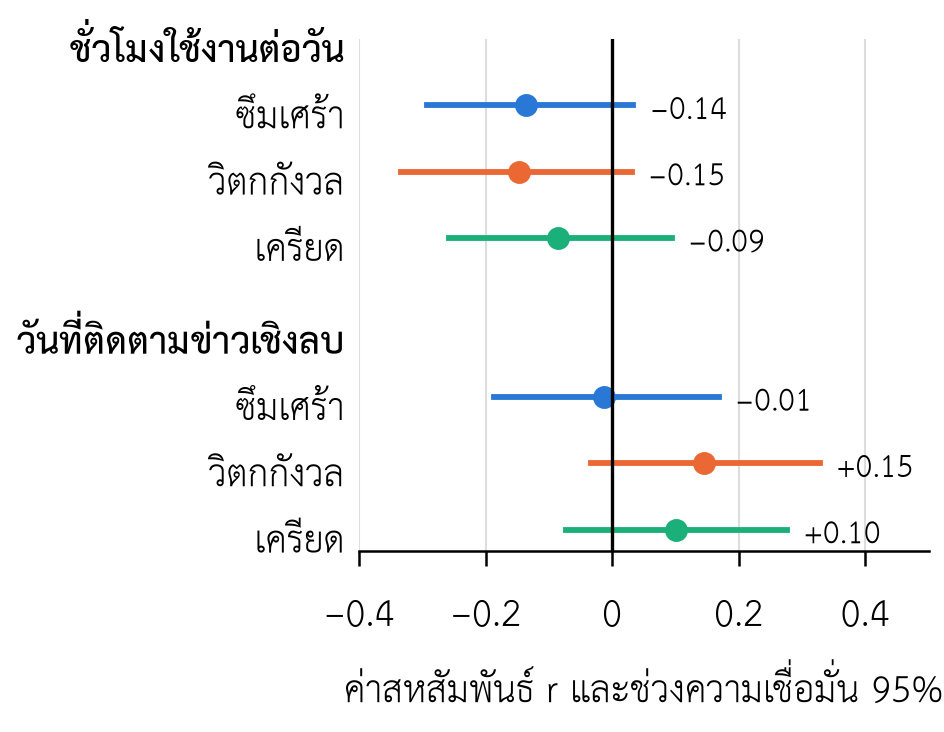
\includegraphics[width=\columnwidth]{fig-correlation.png}
\caption{ค่าสหสัมพันธ์ของชั่วโมงใช้งานและวันที่ติดตามข่าวเชิงลบกับคะแนน DASS-21
         เส้นแนวนอนคือช่วงความเชื่อมั่น 95\% ($n = 107$)}
\label{fig:correlation}
\end{figure}

\subsection{ประเภทเนื้อหาและการนอน}

คะแนนของผู้ที่ดูเนื้อหาต่างกลุ่มกันไม่ต่างกันในทุกมิติ
(Kruskal-Wallis \stat{p}~= 0.936, 0.883 และ 0.691
สำหรับภาวะซึมเศร้า ความวิตกกังวล และความเครียด)
กลุ่มข่าวมีคะแนนความวิตกกังวลเฉลี่ยสูงที่สุด (13.00) เทียบกับบันเทิง 11.59 อื่น~ๆ 11.00
และชีวิตคนอื่น 10.46 แต่ ANOVA ไม่พบความต่าง (\stat{F}(3,~103)~= 0.225, \stat{p}~= 0.879)
ทั้งนี้กลุ่มข่าวมีเพียง 8 คน จึงตรวจความต่างขนาดเล็กได้ยาก

ชั่วโมงใช้โซเชียลมีเดียไม่สัมพันธ์กับชั่วโมงการนอน (\stat{r}~= 0.049, \stat{p}~= 0.616)
และไม่สัมพันธ์กับคุณภาพการนอน (\stat{r}~= 0.114, \stat{p}~= 0.243)
แต่คุณภาพการนอนเองสัมพันธ์ทางลบกับภาวะซึมเศร้า (\stat{r}~= −0.276, \stat{p}~= 0.004)
และความเครียด (\stat{r}~= −0.320, \stat{p}~< 0.001)
ส่วนชั่วโมงการนอนและจำนวนวันที่ออกกำลังกายไม่สัมพันธ์กับมิติใดอย่างมีนัยสำคัญ

\subsection{เมื่อควบคุมปัจจัยอื่น}

ตัวแปรต้นทั้งแปดตัวมีค่า VIF ระหว่าง 1.05 ถึง 1.54
จึงไม่มีปัญหาตัวแปรต้นสัมพันธ์กันเอง
ตาราง~\ref{tab:regression} แสดงว่าตัวแปรโซเชียลมีเดียทั้งสองตัวเพิ่ม \Rsq{} ได้น้อย
และไม่มีนัยสำคัญในมิติใด
มิติความวิตกกังวลเพิ่มมากที่สุด ($\Delta$\Rsq~= 0.045, \stat{p}~= 0.100)
และหลังปรับ Bonferroni ค่า \stat{p} เป็น 0.301

\begin{table}[!t]
\centering\small
\caption{สัมประสิทธิ์ \stat{b} ของการถดถอยพหุคูณแบบลำดับขั้น ($n = 103$)}
\label{tab:regression}
\begin{tabularx}{\columnwidth}{|L|r|r|r|}
\hline
\textbf{ตัวแปรต้น} & \textbf{ซึมเศร้า} & \textbf{วิตกกังวล} & \textbf{เครียด} \\
\hline
ชั่วโมงใช้งานต่อวัน & −0.268 & −0.391 & −0.187 \\
วันที่ติดตามข่าวเชิงลบ & 0.023 & 0.872 & 0.534 \\
ชั่วโมงการนอน & 1.150 & 0.069 & 0.195 \\
คุณภาพการนอน & −0.921* & −0.162 & −0.878* \\
วันที่ออกกำลังกาย & 0.176 & −0.066 & −0.185 \\
ความกดดันจากการเรียน & 0.979** & 0.329 & 0.800* \\
เกรดเฉลี่ยสะสม & −0.706 & −0.958 & 0.115 \\
ความเพียงพอทางการเงิน & −1.125** & −0.663* & −0.626 \\
\hline
\Rsq{} ขั้นที่ 1 & 0.263 & 0.058 & 0.191 \\
\Rsq{} ขั้นที่ 2 & 0.271 & 0.103 & 0.205 \\
$\Delta$\Rsq & 0.008 & 0.045 & 0.013 \\
\stat{p} ของ $\Delta$\Rsq & 0.615 & 0.100 & 0.454 \\
\hline
\end{tabularx}

\vspace{2pt}
\raggedright หมายเหตุ: * \stat{p}~< 0.05, ** \stat{p}~< 0.01 ก่อนปรับ Bonferroni
ค่าความคลาดเคลื่อนมาตรฐานแบบ HC3
\end{table}

ตัวแปรที่มีน้ำหนักในสมการเป็นตัวแปรควบคุม ไม่ใช่ตัวแปรโซเชียลมีเดีย
ในสมการภาวะซึมเศร้า ความเพียงพอทางการเงินมีน้ำหนักมากที่สุด ($\beta = -0.293$)
ตามด้วยความกดดันจากการเรียน ($\beta = 0.269$) และคุณภาพการนอน ($\beta = -0.242$)
เมื่อปรับ Bonferroni แล้ว เหลือเพียงความเพียงพอทางการเงิน (\stat{p}~= 0.002)
และความกดดันจากการเรียน (\stat{p}~= 0.026) ในสมการภาวะซึมเศร้าที่ยังมีนัยสำคัญ
ในสมการความเครียดซึ่งควบคุมเกรดเฉลี่ยและสภาพการเงินแล้ว
สัมประสิทธิ์ของชั่วโมงใช้งานคือ \stat{b}~= −0.187 คะแนนต่อชั่วโมง
(95\% CI −0.71 ถึง 0.34, \stat{p}~= 0.485)
ผู้ที่ใช้โซเชียลมีเดียมากกว่าจึงไม่ได้เครียดต่างจากผู้ที่ใช้น้อยกว่า
การตรวจข้อตกลงเบื้องต้นพบความแปรปรวนไม่คงที่ในสมการภาวะซึมเศร้า
(Breusch-Pagan \stat{p}~= 0.013) ซึ่งเป็นเหตุผลที่ใช้ HC3
และค่าคลาดเคลื่อนของสมการความวิตกกังวลไม่แจกแจงปกติ (Shapiro-Wilk \stat{p}~= 0.001)
จากผู้ตอบไม่กี่คนที่มีคะแนนสูงมาก

\subsection{สภาพการเงิน}

เมื่อแบ่งผู้ตอบตามคะแนนความเพียงพอทางการเงินเป็น 3 กลุ่ม คือ ไม่พอใช้ (1--4) พอใช้ (5--7)
และสบาย (8--10) คะแนนภาวะซึมเศร้าต่างกันมากที่สุด (ภาพ~\ref{fig:finance})
กลุ่มไม่พอใช้มีคะแนนเฉลี่ย 16.6 ขณะที่กลุ่มสบายมี 6.6
(\stat{F}(2,~104)~= 10.91, \stat{p}~< 0.001, \etasq{}~= 0.173, Cohen's \stat{d}~= 1.59)
ความเครียดต่างกันเช่นกัน (\stat{F}(2,~104)~= 5.02, \stat{p}~= 0.008, \etasq{}~= 0.088)
ส่วนความวิตกกังวลไม่ต่างกัน (\stat{p}~= 0.153) และการทดสอบ Kruskal-Wallis ให้ข้อสรุปเดียวกัน
เมื่อใช้คะแนน 1--10 โดยตรง ความเพียงพอทางการเงินสัมพันธ์กับภาวะซึมเศร้า (\stat{r}~= −0.374)
แรงกว่าชั่วโมงใช้โซเชียลมีเดีย (\stat{r}~= −0.136) เกือบสามเท่า
ส่วนเกรดเฉลี่ยสะสมไม่สัมพันธ์กับมิติใด ($|r| \le 0.063$)

\begin{figure}[!t]
\centering
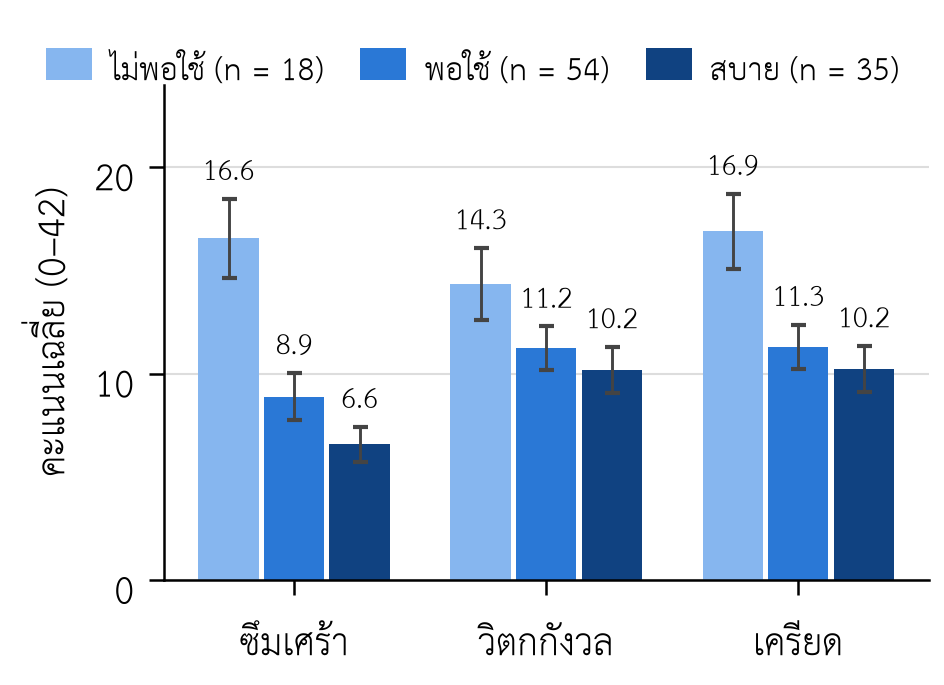
\includegraphics[width=\columnwidth]{fig-finance.png}
\caption{คะแนนเฉลี่ย DASS-21 แยกตามความเพียงพอทางการเงิน ไม่พอใช้ (1--4) พอใช้ (5--7)
         และสบาย (8--10) เส้นบนแท่งคือค่าคลาดเคลื่อนมาตรฐาน}
\label{fig:finance}
\end{figure}

\subsection{ผลเมื่อรวมผู้ที่ไม่ผ่านข้อดักความใส่ใจ}

เมื่อวิเคราะห์ชุดเดิมกับผู้ตอบทั้ง 121 คน ข้อสรุปหลักยังเหมือนเดิม แต่มีผลสองข้อที่เปลี่ยน
คือ สหสัมพันธ์บางส่วนระหว่างการติดตามข่าวกับความวิตกกังวลกลายเป็นมีนัยสำคัญ
(partial \stat{r}~= 0.189, \stat{p}~= 0.047)
และคะแนนภาวะซึมเศร้าของชายและหญิงต่างกันอย่างมีนัยสำคัญ (\stat{p}~= 0.049)
ผลทั้งสองข้อขึ้นกับผู้ตอบที่ไม่ได้อ่านคำถามจริง จึงไม่นำมาสรุป

% 5. สรุปผลและข้อเสนอแนะ -- ย่อจากรายงานบทที่ 5 (../report/chapter/05-conclusion.tex)
% ตัวเลข power คำนวณจากการแปลง Fisher z ที่ alpha = 0.05 สองทาง (เหมือนในรายงาน)
\section{สรุปผลและข้อเสนอแนะ}

\subsection{สรุปผล}

ในนักศึกษา 107 คน ชั่วโมงใช้โซเชียลมีเดียต่อวันไม่สัมพันธ์กับภาวะซึมเศร้า ความวิตกกังวล
และความเครียด ทั้งก่อนและหลังควบคุมปัจจัยอื่น ประเภทเนื้อหาที่ดูมากที่สุดไม่ทำให้คะแนนต่างกัน
และการติดตามข่าวเชิงลบสัมพันธ์กับความวิตกกังวลมากกว่ามิติอื่นตามที่คาดไว้ แต่ไม่มีนัยสำคัญ
ตัวแปรที่สัมพันธ์กับคะแนนชัดที่สุดคือความเพียงพอทางการเงิน
ตามด้วยคุณภาพการนอนและความกดดันจากการเรียน

\subsection{อภิปรายผล}

ผลที่ไม่พบความสัมพันธ์กับเวลาที่ใช้สอดคล้องกับงานของ Orben และ Przybylski
\cite{orben2019association} ซึ่งพบขนาดผลเพียงร้อยละ 0.4 หรือ \stat{r} ประมาณ 0.06
หากความสัมพันธ์จริงมีขนาดเท่านี้ กลุ่มตัวอย่าง 107 คนมีโอกาสตรวจพบเพียงประมาณร้อยละ 10
และต้องใช้ผู้ตอบราว 1,960 คนจึงจะมีโอกาสตรวจพบร้อยละ 80
ผลนี้จึงไม่ได้แปลว่าไม่มีความสัมพันธ์ แต่บอกว่าถ้ามีก็เล็กเกินกว่ากลุ่มตัวอย่างขนาดนี้จะตรวจพบ
นอกจากนี้ ผู้ตอบทุกคนใช้โซเชียลมีเดียอย่างน้อย 4 ชั่วโมงต่อวัน
ช่วงของตัวแปรที่แคบเช่นนี้ทำให้ค่า \stat{r} เล็กลงได้
ผลนี้ยังเข้ากับข้อสรุปของ Sala และคณะ \cite{sala2024umbrella}
ว่าผลไม่ได้ขึ้นกับเวลาที่ใช้อย่างเดียว

ทิศทางของผลเรื่องการติดตามข่าวตรงกับงานของ Dominguez-Rodriguez และคณะ
\cite{dominguez2025climate} แต่ไม่มีนัยสำคัญ เหตุผลที่เป็นไปได้มีสามข้อ
ข้อแรก งานวิจัยนี้วัดเพียงความถี่ของการติดตามข่าว ไม่ได้ใช้แบบวัด doomscrolling เต็มรูปแบบ
ข้อที่สอง มิติความวิตกกังวลมีความเชื่อมั่นต่ำที่สุด ซึ่งทำให้ค่า \stat{r} ที่วัดได้ต่ำกว่าความจริง
ข้อที่สาม ถ้าขนาดผลจริงเท่ากับที่พบ (\stat{r}~= 0.146)
ต้องใช้ผู้ตอบราว 366 คนจึงจะมีโอกาสตรวจพบร้อยละ 80

ความเพียงพอทางการเงินถูกใส่ไว้ในฐานะตัวแปรควบคุม
แต่กลับเป็นตัวแปรที่แยกคะแนนภาวะซึมเศร้าได้ชัดที่สุด
อย่างไรก็ตาม ข้อมูลเก็บครั้งเดียว จึงบอกไม่ได้ว่าปัญหาการเงินทำให้ซึมเศร้า
หรือผู้ที่ซึมเศร้าประเมินสภาพการเงินของตนแย่กว่าความจริง
ส่วนกลไกการแย่งเวลาไม่ได้รับการสนับสนุน เพราะชั่วโมงใช้งานไม่สัมพันธ์กับการนอน
และสิ่งที่สัมพันธ์กับคะแนนคือคุณภาพการนอน ไม่ใช่จำนวนชั่วโมง
ด้านแบบวัด ค่าแอลฟาทั้งฉบับ (0.894) ใกล้กับที่ Manzar และคณะ \cite{manzar2025dass21} รายงานไว้
แต่ภาวะซึมเศร้ากับความเครียดสัมพันธ์กันค่อนข้างสูง (\stat{r}~= 0.68)
การเทียบว่าตัวแปรใดสัมพันธ์กับมิติใดมากกว่ากันจึงต้องตีความอย่างระมัดระวัง

\subsection{ข้อจำกัด}

ข้อมูลเก็บครั้งเดียว จึงบอกได้เพียงความสัมพันธ์ ไม่ใช่เหตุและผล
กลุ่มตัวอย่างเลือกแบบตามสะดวกจากมหาวิทยาลัยเดียว มีจำนวน 107 คน น้อยกว่าเป้า 150 ถึง 200 คน
และกระจุกในชั้นปีที่ 2 (ร้อยละ 81.3) กลุ่มเนื้อหาข่าวมีเพียง 8 คน
ตัวแปรหลายตัวเป็นการรายงานตนเอง และการปรับค่า \stat{p} ด้วยวิธี Bonferroni ทำเฉพาะการถดถอย
ผลการศึกษาใช้ได้ในระดับกลุ่มเท่านั้น ไม่ใช้วินิจฉัยสุขภาพจิตรายบุคคล

\subsection{ข้อเสนอแนะ}

ในการนำผลไปใช้ ข้อมูลชุดนี้สนับสนุนให้การดูแลสุขภาพจิตนักศึกษา
ให้ความสำคัญกับเรื่องค่าใช้จ่ายและคุณภาพการนอนมากกว่าการจำกัดเวลาหน้าจอ
สำหรับการศึกษาครั้งต่อไป ควร
(1)~กำหนดขนาดกลุ่มตัวอย่างจากขนาดผลที่คาดไว้ เช่น อย่างน้อย 366 คนสำหรับเรื่องการติดตามข่าว
(2)~สุ่มตัวอย่างให้กระจายตามชั้นปีและคณะ
(3)~ใช้แบบวัด doomscrolling เต็มรูปแบบ และวัดรูปแบบการใช้งานให้ละเอียดขึ้น
และ (4)~เก็บข้อมูลกลุ่มเดิมซ้ำหลายช่วงเวลา เพื่อดูว่าพฤติกรรมหรืออาการเกิดก่อน


\bibliographystyle{IEEEtran}
\bibliography{ieee-control,../references}

\end{document}
